\subsection{Image experiments}
For the image experiments we collected our dataset by downloading the complete galleries from around 30 artists.
Those artists were selected from the daily deviations of a random day and includes both premium and non premium members.
In total we downloaded around 5000 images. 
For each image we also stored the category information.
The dataset is unbalanced since some artists only have around 50 images, while other artists have over 500 images.
The top five categories are listed in table \ref{datasetstats}.

\begin{table}
    \centering
    \begin{tabular}
        { | l | c | } 
        \hline
        Category & count \\
        \hline
        photography & 2244 \\ 
        customization & 906 \\ 
        traditional & 842 \\ 
        digitalart & 587 \\ 
        fanart & 239 \\ 
        \hline 
    \end{tabular}
    \caption{Dataset category statistics}
    \label{datasetstats}
\end{table}

\subsubsection{Experiment 1: 1 vs all artists}
The first experiment using this toolkit is to find out if there are any artists in our dataset that uses an unique style.
The experiment is performed using two feature combination, the statistical features and the cognitive features.
Also it is focused on using one artist as the positive class while all the other artists are in the negative class resulting in a two class problem.
This experiment is set up as an orientation experiment to find out what might work for this dataset and what might not.
Also this experiment can give a clear indication of how to approach this type of dataset.

For this experiment, three classifiers were used: kNN, Naive Bayes and the Nearest Mean classifiers.
The classifiers were trained on a train set which consists of 70\% of the entire dataset.
Training was done with a 5 fold cross-validation and the performance of each classifier can be computed by calculating the average of the $F_1$-measure gathered from all folds.
Because this is an orientation experiment, no test set was incorporated in this experiment.

\subsubsection{Experiment 1: Results}

\begin{table}
    \centering
    \begin{tabular}
        { | l | l | c | c } 
        \hline
        Artist & Classifier & Parameter & F-Measure \\
        \hline
        my\_shots & Nearest Mean & - & 0.8742 \\ 
        gsphoto & kNN & 3 & 0.8722 \\ 
        gsphoto & kNN & 5 & 0.8711 \\ 
        Pierrebfoto & Naive Bayes & 10 & 0.8698 \\ 
        Kitsunebaka91 & Naive Bayes & 24 & 0.8693 \\
        Kitsunebaka91 & Naive Bayes & 12 & 0.8680 \\
        gsphoto & kNN & 7 & 0.8669 \\
        Kitsunebaka91 & Naive Bayes & 22 & 0.8668 \\
        gsphoto & kNN & 9 & 0.8664 \\
        Kitsunebaka91 & Naive Bayes & 8 & 0.8657 \\
        \hline 
    \end{tabular}
    \caption{Top 10 Ranking of the highest $F_1$-measure using \textit{statistical features}}
    \label{ex1aresults}
\end{table}

The results from the experiment for the statistical features can be found in table \ref{ex1aresults}.
The table lists the top 10 ranking of the artist names combined with the classifier and parameter used to train the classifier.
The ranking is in a descending order starting from the combination that performed the best according to the $F_1$-measure.

The table shows that 2 artist names exists multiple times in the top 10 ranking.
Those artists are \textit{Kitsunebaka91} and \textit{gsphoto} and the table shows that they were separated from all other artists using different classifiers and parameter settings.

The table also shows that the nearest mean classifier only has one entry in the top 10.
Eventhough it has the highest $F_1$-measure, the classifier does not seem to be performing well on the other artists.

\begin{table}
    \centering
    \begin{tabular}
        { | l | l | c | c } 
        \hline
        Artist & Classifier & Parameter & F-Measure \\
        \hline
        giannisgx89 & Nearest Mean & - & 0.8549 \\ 
        gsphoto & Nearest Mean & - & 0.8196 \\ 
        Pierrebfoto & Nearest Mean & - & 0.7305 \\ 
        sekcyjny & Nearest Mean & - & 0.7298 \\ 
        fediaFedia & Nearest Mean & - & 0.7133 \\
        NEDxfullMOom & Nearest Mean & - & 0.7020 \\
        erroid & Nearest Mean & - & 0.6831 \\
        gsphoto & Naive Bayes & 14 & 0.6820 \\
        Mentosik8 & Nearest Mean & - & 0.6801 \\
        gsphoto & Naive Bayes & 10 & 0.6753 \\
        \hline 
    \end{tabular}
    \caption{Top 10 Ranking of the highest $F_1$-measure using \textit{cognitive} features}
    \label{ex1bresults}
\end{table}

Table \ref{ex1bresults} shows the results obtained from only using cognitive features to separate artists from each other.
In contrast to table \ref{ex1aresults} these results show that the nearest mean classifier is the one having the best performance according to $F_1$-measure.

However using cognitive features results into a different ranking of separable artists, the performance of each classifier is not as high as for using statistical features.
The top 10 ranking using the statistical features all have scores above the 0.8 indicating that using statistical features seems more stable compared to using cognitive features.

This orientation experiment showed that using statistical features better results can be obtained compared to using cognitive features.
Also it seems like there are some artists that can be seperable from all the others but most artists do not perform well in this experiment.
Using the results of this experiment it is hard to describe why this is happening. 
An experiment showing which features contributes to the separation of an artist from all other artists is important in order to describe why the style of an artist is unique compared to the other artists in the dataset.
The next section describes an experiment that gives a clear view over these questions.

\subsubsection{1 vs 1 artists - classification performance}
The real experiment must give a message that this toolkit and deviantart is an interesting research area.

\subsection{Network experiments}
dataset

small world, describe network, identify core

\begin{figure}[htb]
  \centering
  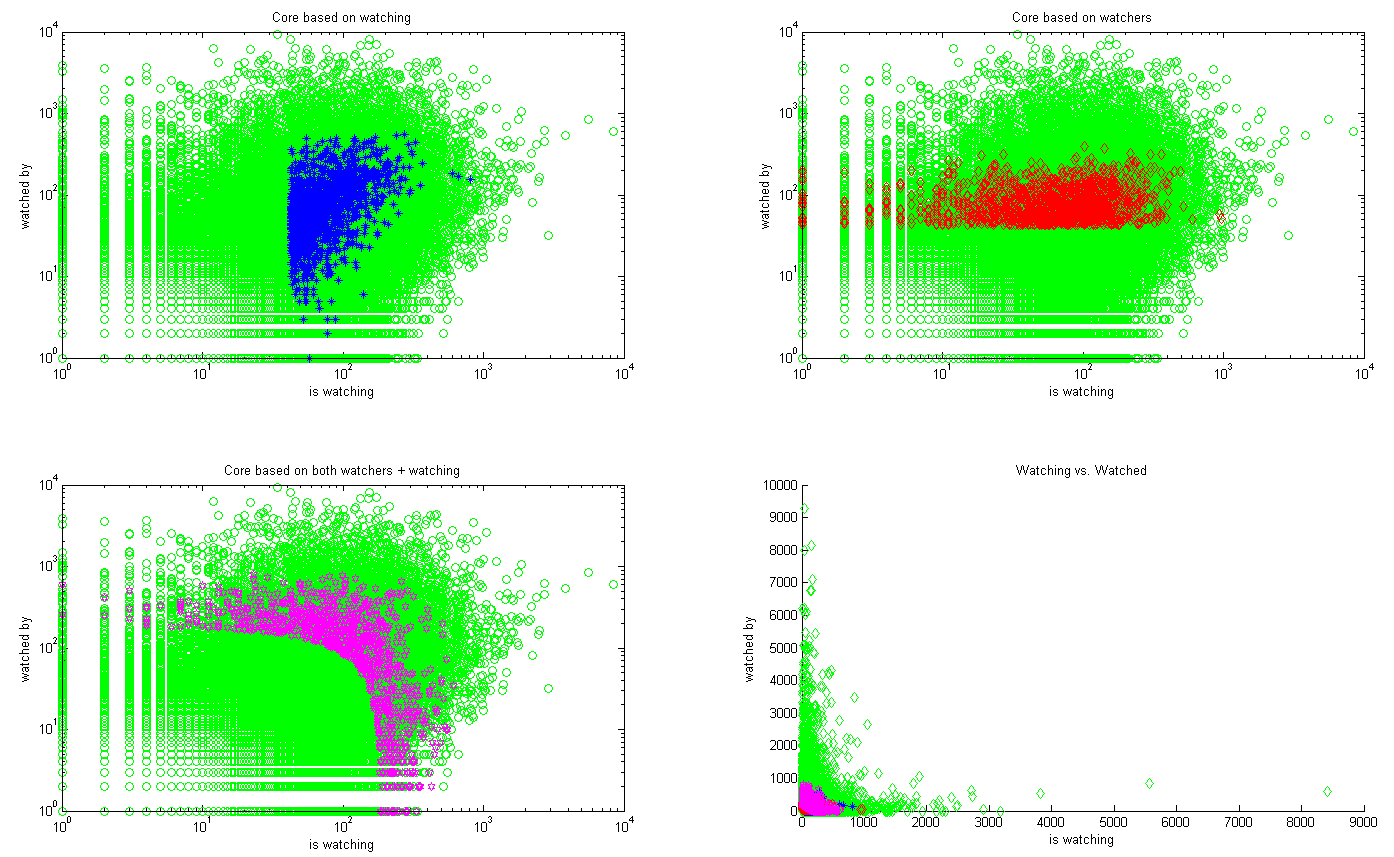
\includegraphics[width=1\linewidth]{img/core.png}
  \caption{Core network}
  \label{fig:results_core}
\end{figure}